%%%%%%%%%%%%%%%%%%%%%%%%%%%%%%%%%%%%%%%%%%%%%%%%%%%%%%%%%%%%%%%%%
%%%  Capstone Project Template that tries to save a few trees %%%
%%%  Edwin Blake 22 Aug 2013                                  %%%
%%%		1 Aug 2014 (revised)                          %%% 
%%%             10 Aug 2015                                   %%%
%%%  see also                                                 %%%
%%% http://ravirao.wordpress.com/2005/11/19/latex-tips-to-meet-publication-page-limits/  
%%%%%%%%%%%%%%%%%%%%%%%%%%%%%%%%%%%%%%%%%%%%%%%%%%%%%%%%%%%%%%%%%

\documentclass[11pt,a4paper]{article}
\usepackage{times}
\usepackage{fancyhdr}           % Allows better control over headers and footers
%\usepackage{layout}            % use with \layout to see the page layout for
%debugging purposes.
\usepackage[margin=2.5cm]{geometry}  %   set the margins using the
                                %   geometry package (which is much
                                %   the easiest way of doing this).
\usepackage[pdftex]{graphicx}   %   Pictures (means you have to
                                %   produce pdf output via pdflatex)
\usepackage[small,compact]{titlesec}   % Try to reduce the white space
                                % latex loves so much
\titlelabel{\thetitle. \quad}   % Reduce space around section heads
                                % and add a full stop after the number
\pagestyle{fancy}               % Invoke fancy headers

\renewcommand{\abstractname}{\vskip -5mm}  %  Change name of Abstract
                                %  to nothing and loose some of the
                                %  excessive white space
\begin{document}

\title{Guidelines for Capstone Project Report\\Using \LaTeXe} \date{}
\author{Clayton Sibanda\\Department of Computer Science\\SBNCLA002@myuct.ac.za
\and David Kheri\\Department of Computer Science\\KHRDAV001@myuct.ac.za
\and Meluleki Dube\\Department of Computer Science\\DBXMEL004@myuct.ac.za}

%%%  Set the headers via fancyhdr package
\lhead{Capstone Project Report using \LaTeXe}  % Short title for running head
\chead{}
\rhead{1st August, 2014}   %  Fixed running head of the date
\lfoot{}
\cfoot{\thepage}    %  add page number as centre footer.
\rfoot{}
\renewcommand{\headrulewidth}{0.0pt}   % Don't want horizontal line
                                % under header.

\maketitle
\thispagestyle{plain}  % First page is plain style headings and
                       % footers (ie just the page number as footer).

\begin{abstract}
  This document outlines the requirements for the final report for the
  Computer Science Capstone Project Report and describes the use of
  the \LaTeXe for that purpose. Please follow this precise template
  for your final report.
\end{abstract}

\section{Introduction}
The capstone project is done as the culmination of your three year
study of Computer Science. It is the development of a real application
that draws on all your knowledge of the field gained in the course of
your training in the subject.

The project should be written up as a professional software
engineering design and development project. We expect a report of
about 3500-4000 words, written single spaced, with a font size of at
least 11 pts. Use at least a 2.5 cm margin on all sides of the
pages. Please use ``styles'' for formatting if you are using a word
processing package or use \LaTeX. We mean you to use styles for
everything, not just headings and lists but also for a different
font. So use emphasis for \emph{italics} and do \emph{not} use a bold
face. No blank lines between paragraphs except to get figures and
their captions to position properly.

Depending on how many diagrams you use (more is better) the report
will be between 7 and 10 pages long. Note that while word users will
struggle with numbered headings and lists, \LaTeX\/ has its own ideas
about where ``floats'' (like tables and figures) will go, as usual
search the internet for advice (e.g., search for ``\LaTeX quick
guide'' and look at
http://www.andy-roberts.net/writing/latex/floats\_figures\_captions). Don't
worry, word's specialty is loosing your figures in some between-page
limbo; \LaTeX\/ will not loose them, just place them way after the
spot where you want them.  This document shows the format we expect
and you can use it as a template.  Your appendices (e.g., user manual,
test results, which are needed) are not included in these limits.

You must had-in an Adobe Acrobat file for your report (i.e., pdf
file). Not word, latex source, but \emph{PDF}!


\section{Approach}
You should begin your write-up with an overview and then drill down
into the details of what you produced. Your report should cover the
following sections (Sections \ref{ss:introduction} --\ref{ss:conclusion}).

%Clayton
\subsection*{Abstract}
First you should have an executive summary (or abstract) just a single
paragraph saying what the results of the project are (at most 200
words).

%Clayton
\subsection{Introduction}
\label{ss:introduction}

Your introduction provides the context for the project and should
contain the statement of the scope of the project (which may have
changed since you first wrote it). Someone reading your introduction
must have clear idea of what the system is intended for. If you think
there is something special about the kind of problem you tackled that
your reader needs to know up front then this is where you say it.

If you need any survey of other work (you probably don't) then put it
towards the end of the introduction and give suitable references. A
case where this is needed is if your project builds on someone else's
project or some published algorithm.

Discuss your approach to solving the problem. Please give a short
overview of the software engineering methods you used (e.g.,
traditional analysis followed by design and implementation -- typically
the case if you did an evolutionary prototype, or a more agile
approach where you had a cyclical development process). 


%Meluleki Dube
\section{Requirements Captured}
The following are requirement divided into functional and non-functional requirement which where collected after consulting with the client.
\subsection*{Functionality requirements}
The list of the requirements for the application where as follows:
\newline\textbf{Functional Requirements}
\begin{itemize}
	\item Rendering of the map on the user screen
	\item Have signal strength indicators on the map. These should be updated on a real-time basis.
	\item Save signal strength on the database for a specific location.
	\item Zoom in and zoom out of the campus map
\end{itemize}
\textbf{Non-Functional Requirements}
\begin{itemize}
	\item Real-time receiving of data being updated in the database.
	\item Speed up on the rendering of the areas and their strengths on the map.
\end{itemize}
\subsection*{Use case}
Below is a use case diagram to show the different operation that can be done on the system and the actors who are responsible for performing these actions. Firstly, there is a need to discuss the different users of the systems and the different systems that are used by our system. These make up the actors involved in the system. The different actors and their level of interaction with the application are listed below:
\newline\textbf{Primary Actor}
\begin{itemize}
	\item User
	\item ICTS (extending User)
	\item Phone
\end{itemize}
\textbf{Secondary users}
\begin{itemize}
	\item Server (where the application data )
	\item User (for some instances.)
\end{itemize}
\pagebreak
\begin{figure}
	\centering
	\includegraphics[width=0.7
	\linewidth]{"images/Use Case"}
	\caption{Showing the use case diagram of the Wi-Fi Mapper}
	\label{fig:use-case}
\end{figure}
The main use case for the system is update WLAN Zone information as it is the spawns many more functions that influence the user's view of the menu. The detailed flow of events for updating information of a particular zone are shown by the use case narrative below:
\newline
\begin{tabular}{|p{0.21\textwidth}|p{0.3\textwidth}|p{0.24\textwidth}|p{0.25\textwidth}|}
	\hline
	\textbf{Use Case:} & Update WLAN Zone & \textbf{ID:} 007 & \textbf{Level:} High
	\\\hline
	\textbf{Actors:} & \multicolumn{3}{|l|}{Users, ICTS, Wi-Fi Mapper Server} \\\hline
	\multirow{2}{0.2\textwidth}{\textbf{Stakeholders and Interests}} &
	\multicolumn{3}{|p{0.79\textwidth}|}{
		Josiah Chavula -The owner of the product,
	} \\
	& \multicolumn{3}{|p{0.79\textwidth}|}{
		ICTS - they use the information provided by the system.
	} \\\hline
	\textbf{Brief Description:} & \multicolumn{3}{|p{0.79\textwidth}|}{
	A user who is using the app opens the application to get the different eduroam strength signals. The system gives user the data for the whole UCT upper campus map. If location permissions are granted the user is then also able to send their data to the server and get the map zoomed in to give them strength signals on a few meters radius around them.} \\\hline
	\multirow{2}{0.2\textwidth}{\textbf{Preconditions:}}
	& \multicolumn{3}{|p{0.79\textwidth}|}{
		User connected to eduroam.} \\
	& \multicolumn{3}{|p{0.79\textwidth}|}{
		User is at the locations that are supported by the application.} \\\hline
	\multirow{3}{0.2\textwidth}{\textbf{Post Conditions:}}
	& \multicolumn{3}{|p{0.79\textwidth}|}{Data is updated at the server.} \\
	& \multicolumn{3}{|p{0.79\textwidth}|}{User has a data showing different signal strengths across the UCT Campus.}  \\\hline
	\multirow{1}{0.2\textwidth}{\textbf{Related Use Cases:}}
	& \multicolumn{3}{|p{0.79\textwidth}|}{includes: Get user permissions} \\\hline
\end{tabular}

\begin{longtable}{|p{0.5\textwidth}|p{0.5\textwidth}|}\hline
	\multicolumn{2}{|p{1.095\textwidth}|}{\textbf{Typical Course of Events}} \\\hline
	\textbf{Actor Action} & \textbf{System Response} \\\hline
	\begin{enumerate}[series=typical]
		\item Phone Queries the database for data for the supported areas and return to user. 
	\end{enumerate} &
	\begin{enumerate}[resume=typical]
		\item Queries the database for data for the supported areas and return to user
		\item Request user to give location permissions
	\end{enumerate}
	\\\hline
	\begin{enumerate}[resume=typical]
		\item Grants the system permission to use Location services
	\end{enumerate} &
	\begin{enumerate}[resume=typical]
		\item Get the current user location
		\item Get the signal Strength of the users Wi-Fi
		\item Set up Location Change listener
	\end{enumerate}
	\\\hline
	\begin{enumerate}[resume=typical]
		\item Continuously send the system data from where they are located.
	\end{enumerate}
	&
	\begin{enumerate}[resume=typical]
		\item Constantly accepts data from the users 
		\item Save the data
		\item Use aggregate data from the users to calculate average strength signals for different locations.
	\end{enumerate} \\\hline
	\begin{enumerate}[resume=typical]
		\item User changes zoom level
	\end{enumerate}
	& 
	\begin{enumerate}[resume=typical]
		\item System changes the focus level for the specific area.
	\end{enumerate}
	\\\hline
\end{longtable}

\begin{longtable}{|p{0.5\textwidth}|p{0.5\textwidth}|}\hline
	\multicolumn{2}{|p{1.095\textwidth}|}{\textbf{Alternative Courses of Events}} \\\hline
	\textbf{Actor Action} & \textbf{System Response} \\\hline
	\begin{enumerate}
		\setcounter{enumi}{3}
		\item 
		\begin{enumerate}[series=abnormal0]
			\item Refuse to give the system location permissions
		\end{enumerate}
	\end{enumerate}
	&
	\begin{enumerate}[series=abnormal0]
		\setcounter{enumi}{4}
		\item
		\begin{enumerate}
			\item Continue showing the user the upper campus map without giving them information about where they are. 
		\end{enumerate}
	\end{enumerate} \\\hline
	\begin{enumerate}
		\setcounter{enumi}{7}
		\item 
		\begin{enumerate}[series=abnormal1]
			\item User loses signal to send data to the server
		\end{enumerate}
	\end{enumerate}
	&
	\begin{enumerate}
		\setcounter{enumi}{8}
		\item 
		\begin{enumerate}
			\item User loses signal to send data to the server
			\item System notifies user that disconnection occurred
		\end{enumerate}
	\end{enumerate} \\\hline
\end{longtable}
\begin{figure}
	\centering
	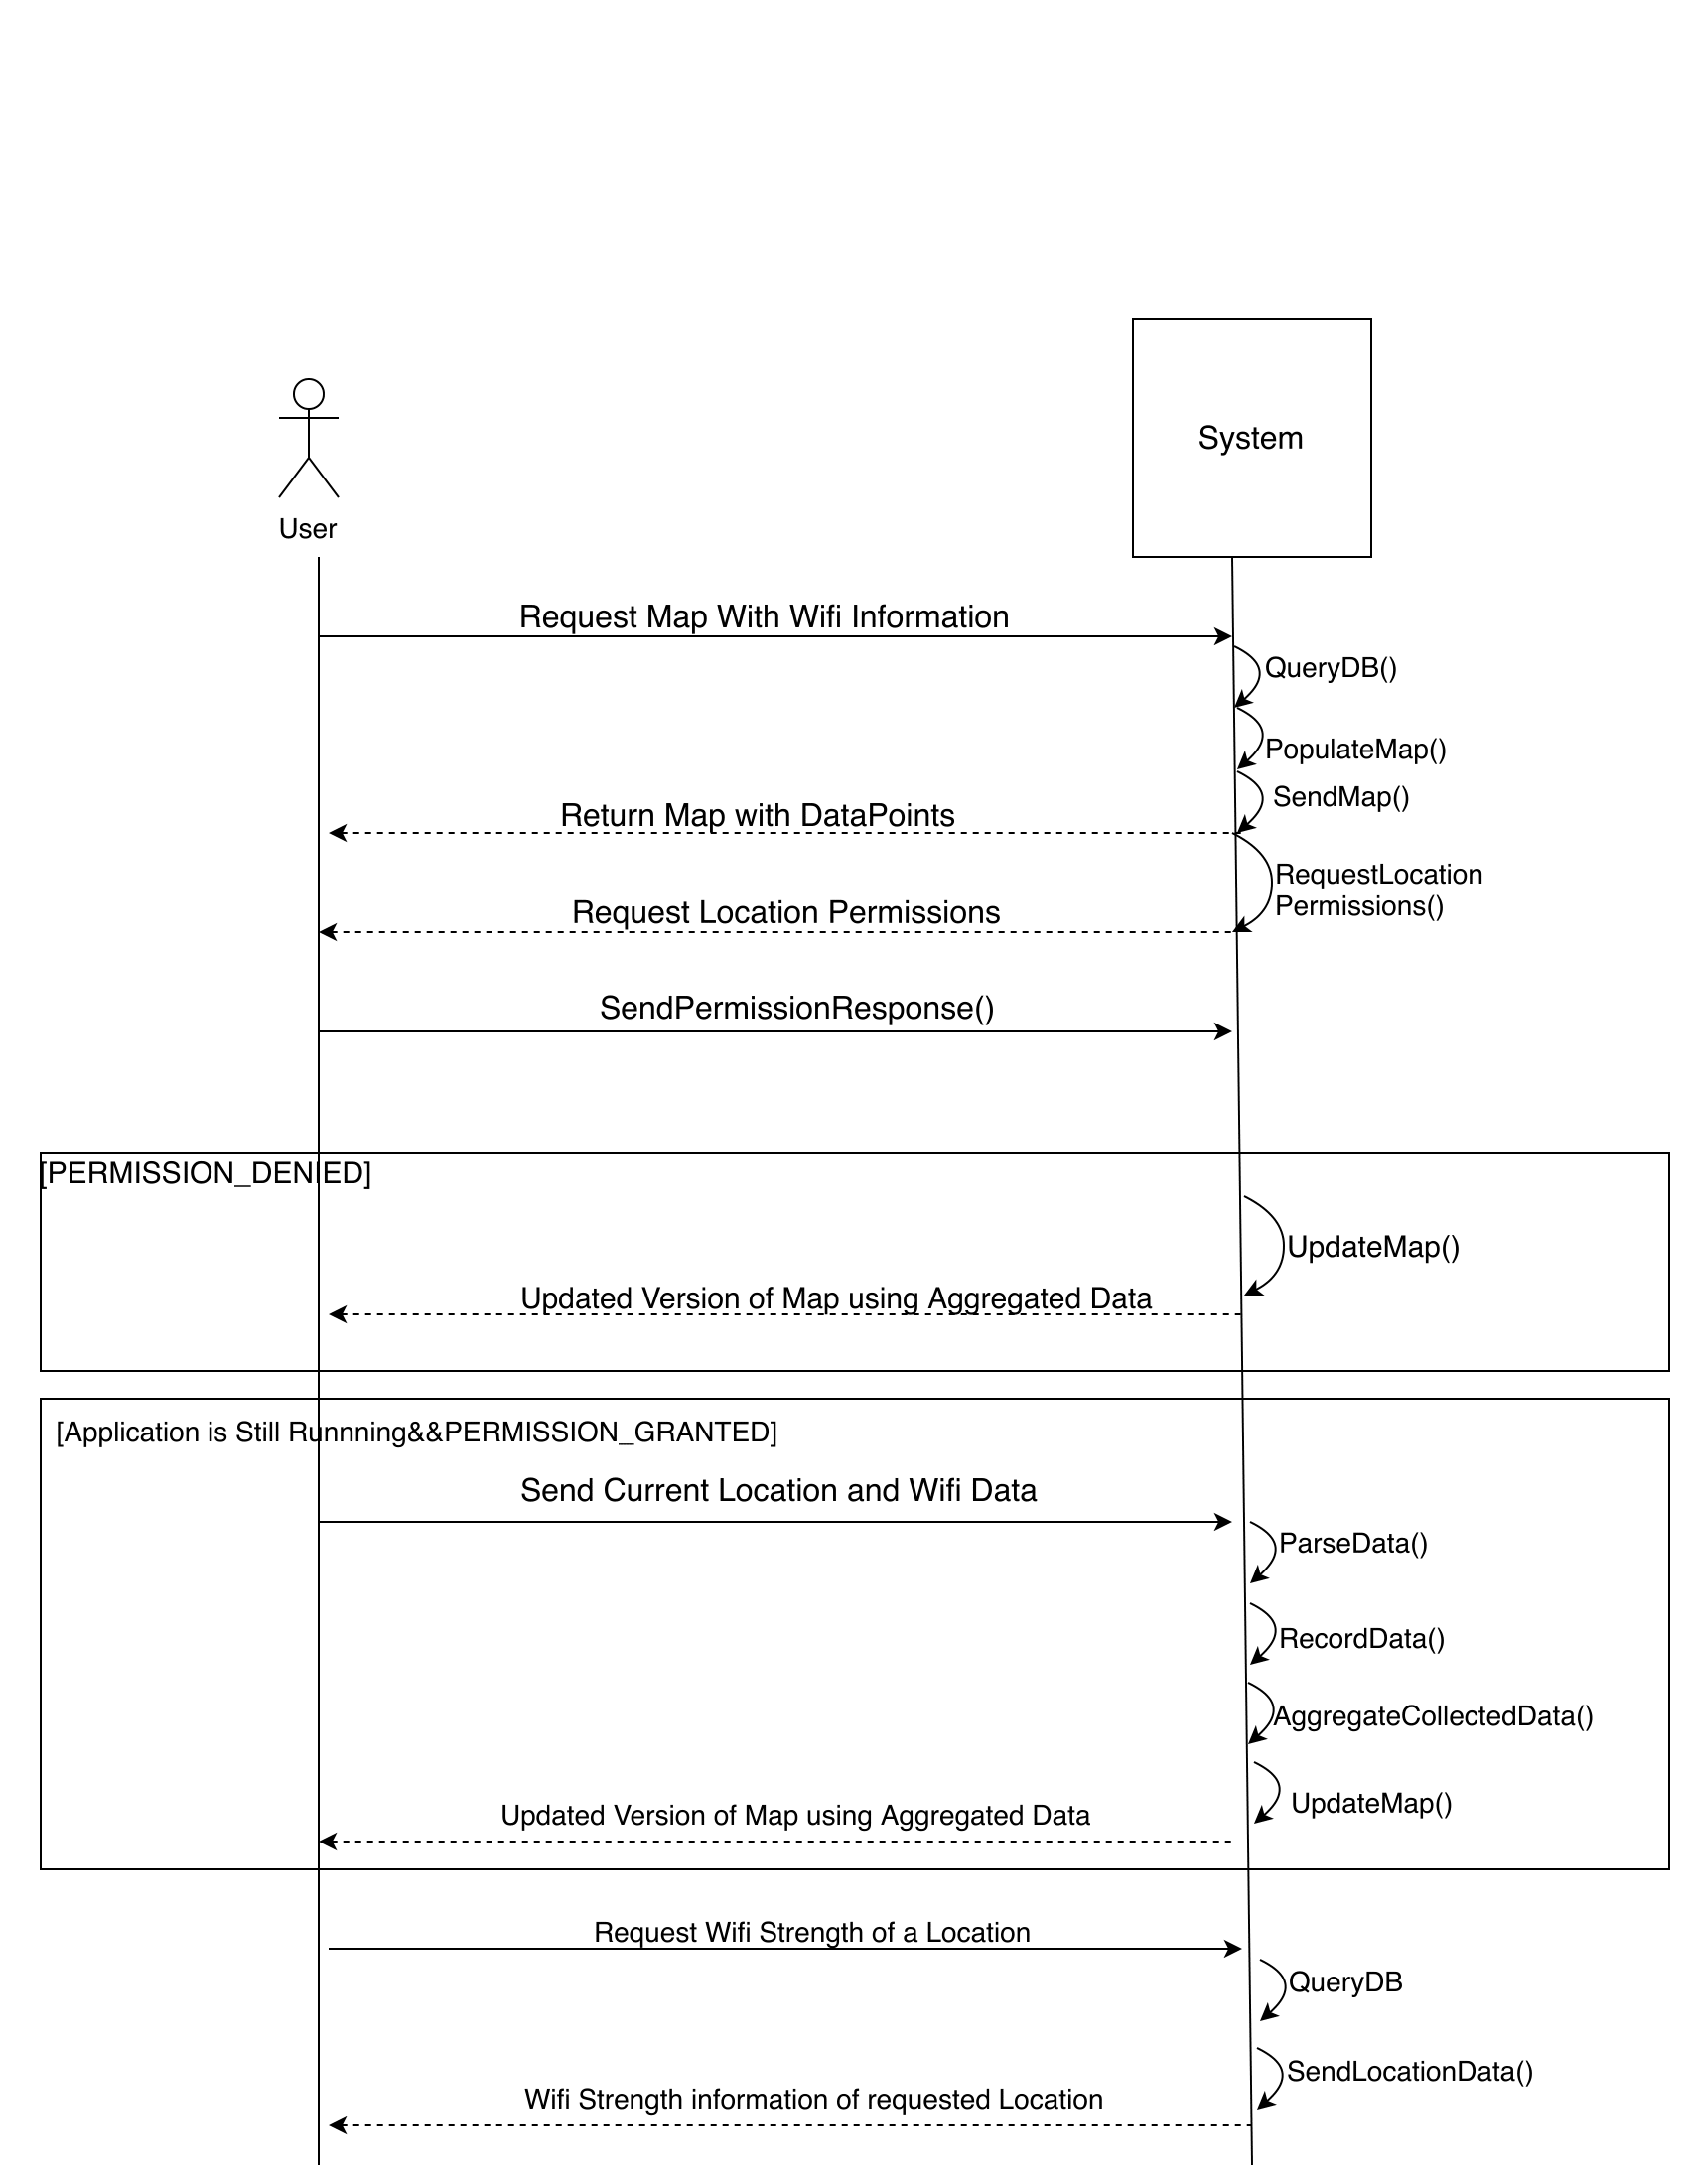
\includegraphics[width=0.7\linewidth]{images/SeqDiagram_Wifi_Mapper}
	\caption{Sequence Diagram}
	\label{fig:seqdiagramwifimapper-1}
\end{figure}

\newpage
\subsection*{Design Overview}
\label{ss:design-overview}
\paragraph{}This Section gives an overview of the system which entails showing how the system interacts with other systems in delivery of functionality to the user and introduce the basic functionality expected from the System,It will also describe what type of stakeholders will interact with the system and what functionality each should expect.

\paragraph{}They are mainly Two ways users can interact with the System that is through a mobile Application(Android Only) and Web Application.

\paragraph{}Mobile Application will need to communicate with the phone's GPS system so as to obtain a user's Location.The functionality provided by GPS is crucial as it pinpoints exactly which WLAN Zone data is collected and ensures accurate aggregate Data is displayed on each WLAN zone.

\paragraph{}Wifi Manager will also be needed by the mobile application so as to obtain Wifi Strength of the router to which the mobile phone is connected to a certain point in time,as both the Wifi Strength and Location to which this data is obtained are the main pieces of information driving the System.

\paragraph{}Since this is a data-centric Application,that means data needs to be stored in a database,both Web Application and Mobile Application will communicate with the database but in slightly different ways.Mobile Application will both query and send data to and from the database while
the web Application will be restricted to just querying data from the database for displaying purposes.

\paragraph{}Query Manager is used by both Mobile so as to validate the data collected corresponds to a WLAN zone or else its not written to the database and handles requests of data from both web and Mobile Application to obtain data to display.

\paragraph{}Both Mobile and Web Application use the Mapping System so as to display a Map to the user which includes data collected from the users stored in the database aggregated into different WLAN zones so as to provide appropriate information to the user.

\paragraph{}Cluster System is required by the Mapping System so as to cluster Data points collected which are very close to each other so as to prevent clutter on the Map which is undesirable to the user(Clustering occurs only at high zoom level).  

\paragraph{}Reporting system is used by the Web Client to generate a report which will provide useful information based on the collected data stored in the database.   
 
\begin{figure}
	\centering
	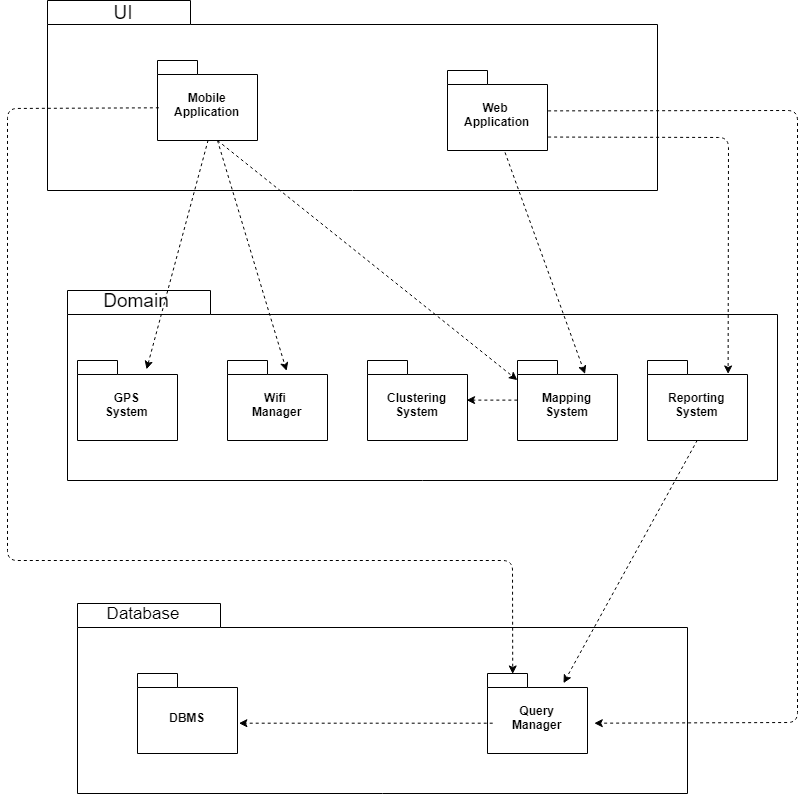
\includegraphics[width=0.7\linewidth]{images/Architecture}
	\caption{Architecture Diagram}
	\label{fig:architecture}
\end{figure}


%Meluleki Dube
\newpage
\section{Implementation}
The major components of the application included, the database, the phone application and the web application version of the application. The application was implemented without a server. The implementation included a cloud database hosted on a third party computer in this case firebase. The phone application was developed for android phones to target the majority of users on campus as per the client's requirements. The Android application was therefore created in Java. The web application was created using JavaScript. Below follows the discussions of these components together with how the they came about and why they were settled on.

\subsection*{Database}
Firebase, a NoSQL cloud database was used as the database option. 
Since a NoSQL database was used, this means that the data in the database was stored as large JSON documents. This helped in reduce the number of deliverable that were to be delivered and hence aided in helping the developers put more focus into other aspects of the problem spectrum. This also reduced the number of resources required to complete the project. The alternative to this would have required a server and a database. The server would have required to be constantly monitored and always on taking data from users and updating it on the database as well as sending new data to the users. With the current approach, we only have a cloud-hosted database that is hosted on Google servers that both applications will be getting data from and sending data to. The database will handle the updating of all users currently connected to it with the new relevant information and as well on the users request give provide the users with the data to populate the menu. The advantages of this approach include the following:
\begin{itemize}
	\item There is no need for a server since firebase database will be able to act both as a server and as a persistent storage tool at the same time. It will assume the role of the server when it needs update the other clients connected to it of new data changes or send the client the data on the database on opening of the application so as to populate the map. This also means there is no stressing about the hosting environment also.
	\item Firebase provide the connected users with realtime updates. This implies that when a value is updated by one user will be sent immediately to the other connected users.
\end{itemize}
\subsubsection*{Database Design}
 During the development cycle, the database had two main designs that where showed to the client. The first design was based on the miscommunication of the client requirements. In this design, the database only stored Location objects together with the signal strengths recorded for that location were stored. This is shown in the figure below
 \begin{figure}
 	\centering
 	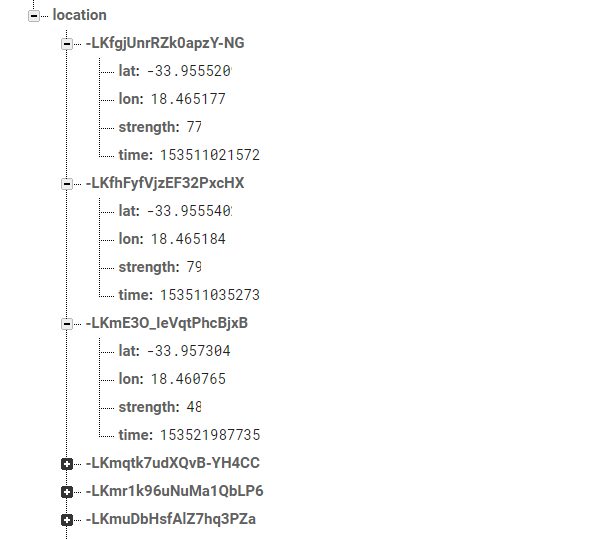
\includegraphics[width=0.7\linewidth]{images/first_db}
 	\caption{Showing the first design of the database developed.}
 	\label{fig:firstdb}
 \end{figure}
As can be seen, there is not much structure in the way the was being stored. Each record had to have an id which made it unique so as to allow better queries. A time stamp was also added to the records on when being written to the database so as to allow future features to use it when they want to filter the strengths based on time. The location was stored as longitude and latitude objects.
\paragraph{}The new database design now also include zone/area objects being stored. This store a list of 4 coordinates that define an area,  the average strength of that area based on location points that are under that area that have recorded data, and lastly the name of the area. This design is shown below in next figure.
\begin{figure}
	\centering
	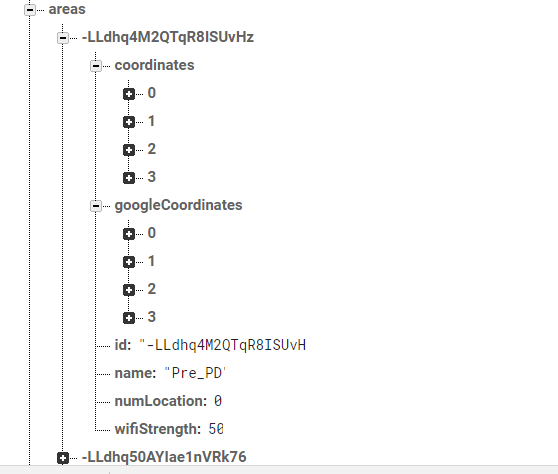
\includegraphics[width=0.7\linewidth]{images/2nd_db}
	\caption[]{Showing the added document for storing area objects.}
\end{figure}
The initial design was still used to maintain the list of all locations that have had data recorded from so as to be able to give the view of the places where the data was recorded for a WLAN zone if needed
Now we get to the details. 

\subsection*{Android application}
The android application was written in Java using the Android Studio tools. The minimum Android version supported in the application was Android 5 API level 21. This version for android was installed in atleast 71\% of the phones of people using android. The reason it was selected to be the minimum supported version was to manage to reach a large population of people at the same time taking advantage of the new features that are in the new APIs which may include better management of resources and security issues for instance. The application built had only one Activity which was the main activity as well. This activity consisted of a map of UCT segmented into different areas based on the buildings and has each color with a specific color that relates into the signal strength in that area. 

\begin{itemize}
\item Describe your data structures and be sure to illustrate them
  with a diagram.

\item If your user interface was a key feature describe how that was
  implemented.

\item Discuss the function of the most significant methods in each
  class. This may well require flowcharts, or sequence diagrams, in
  some cases.

\item Any special relationship between the classes (e.g. friends) and
  why they exist.

\item A description of any special programming techniques or libraries
  used.
\end{itemize}

\subsection*{Web Application}
Wifi mapper comes with a web client that consists of three views and these are map view, login view and the report view.  

The technologies used to build the app are HTML,CSSS and JavaScript. A few frameworks were also include to improve team productivity.

The map view displays a google map that contains the WLAN ZONEs over UCT upper campus. The app gets the map from the google map api obtained by including a script on the html file of the view.

The map view is set up such that the map fills the screen of the device fully. After rendering the map, the app asynchronously gets data from the firebase database using the 'on' firebase listener. The app sets the location center and defualt zoom. In order to get the data from the database firebase was added as a dependence on the app. 

After obtaining the data from the database, the app displays colored polygons on top of respective WLAN ZONEs. The colors of the polygons are calculated using the data returned by the database. Five colors are used to represent ranges between 0 and 100. 

The map view also contains a button used to generate report for special users. On clicking this button, the login view is displayed on the screen.

The login view consists of a login form with two input fields and a login button. The two input fields are for username and password. The password input field is such that the password is hidden while the user is typing it. 

The login button has an onLogin listener attached to it. When the button is clicked/tapped an onLogin event is fired that sends a request to the server to check if the user is authenticated to view the report. If the user is authenticated then the app displays the wifi mapper report.

The report is used to display special statistics to the user. The app calculates the number of locations and signal strength then displays them at the top of the view. Number of WLAN ZONEs is also calculated and displayed together with the number of locations.

Following the calculated numbers, the report displays bar ,pie and bubble charts for the data on firebase. The first bar chart shows the average wifi strength against the WLAN ZONEs on the map. The bar chart is followed by a pie chart that shows a different representation of the average wifi strength against the WLAN.

The app uses a library called chart.js to convert the data from javascript objects to charts. Calculations for the color are done by a single function for all the charts. The calculation is such the only bright colors are used for all chart components.

The report view was developed using modern frameworks like bootstrap that makes the report responsive accross all devices.


%David
\section{Program Validation and Verification}
\label{ss:progr-valid-verif}


WiFi mapper consists of two apps, and these are android app and web app. In order to examine the behaviour of the android app, it was tested on three devices. Upon installing the app, the users, moved around upper campus to collect data at different locations. This was done to test if the app was able to collect data from routers.

<<<<<<< HEAD
For each device that the app was installed, data points were saved on the database. The app also displayed the respective polygons on each WLAN zone across all the devices as the data was collected. This together with other functionalities proved that the app. To test the web app functionalities, the app was deployed and hosted on firebase.

Different devices were used to access the app and it displayed expected across all decices in a responsive manner.

=======
\begin{table}[h!]
  \centering
\caption{Summary Testing Plan. A table caption goes above the table.}
\begin{tabular}[t]{|p{8cm}|p{7cm}|} \hline
  \textbf{Process} & \textbf{Technique} \\ \hline 1. Class
    Testing: test methods and state behaviour of classes & Random,
    Partition and White-Box Tests \\ \hline 2. Integration Testing:
    test the
    interaction of sets of classes & Random and Behavioural Testing \\
    \hline 3. Validation Testing: test whether customer requirements
    are satisfied & Use-case based black box and Acceptance tests \\
    \hline 4. System Testing: test the behaviour of the system as part
    of a larger environment & Recovery, security, stress and
    performance tests \\ \hline
>>>>>>> dbdcaa9c489184e6c0f3ec2628a1dc42bc14dddc


Trello was used to create and manage a test plan for the WiFi mapper project. A board that consisted of items to be tested was created. Each item had a deadline attached to it.This board consisted of features that had been developed but were now waiting to be tested. Another board for items that were in the process of being tested so as to track the items  that were currently being tested. The last board that consisted of items on which testing had already been done was created.

To test each item different testing methodologies were used.

\subsection*{User Interface Testing}
To test the interaction of the user with the app, User Interface testing was used.This was done so as to test the user's interaction with the software. Different navigation functionalities on the map were tested and these involved zooming and panning on the map. Different users were given a running app, the behaviour of the app was noted as the users interacted with the software.User Interface testing ensures that the objects within the user interface function as expected and conform to required standards.

\subsection*{Database Testing}
Database models were tested so as to obtain proper database structure. Writing and querying of the database were also tested. For writing the app was tested for possible race conditions when the app is writing to the databse. For reading the queried data was compared with the expected output.

\subsection*{Unit testing}
To test all methods of objects unit testing was done. Unit testing ensured that all parts of the app are working as expected. To test static methods mock up for testing was used.

\subsection*{Volume Testing}
This kind of testing concerns testing the software for large amounts of data. This test was necessary for wifi mapper as the app keeps on collecting data on many different points. To perform this test multiple clients were used to collect data different points at the same time. As the app receive multiple data the its behaviour was noted.

\subsection*{Security and Access Control Testing}
Application security ensures that proper protection and integrity of data is ensured for all the users. WiFi mapper provides advanced user with private data. As a result the app did require such form of testing.

\subsection*{Failover and Recovery Testing}
Failover testing ensures that, for those systems that need to be kept running, when a failing condition occurs, then the alternate systems properly take over for the failed system without any severe loss of data or transactions. Being a near real-time app, wifi mapper needed to quickly from any failure events.

\begin{figure}
	\centering
	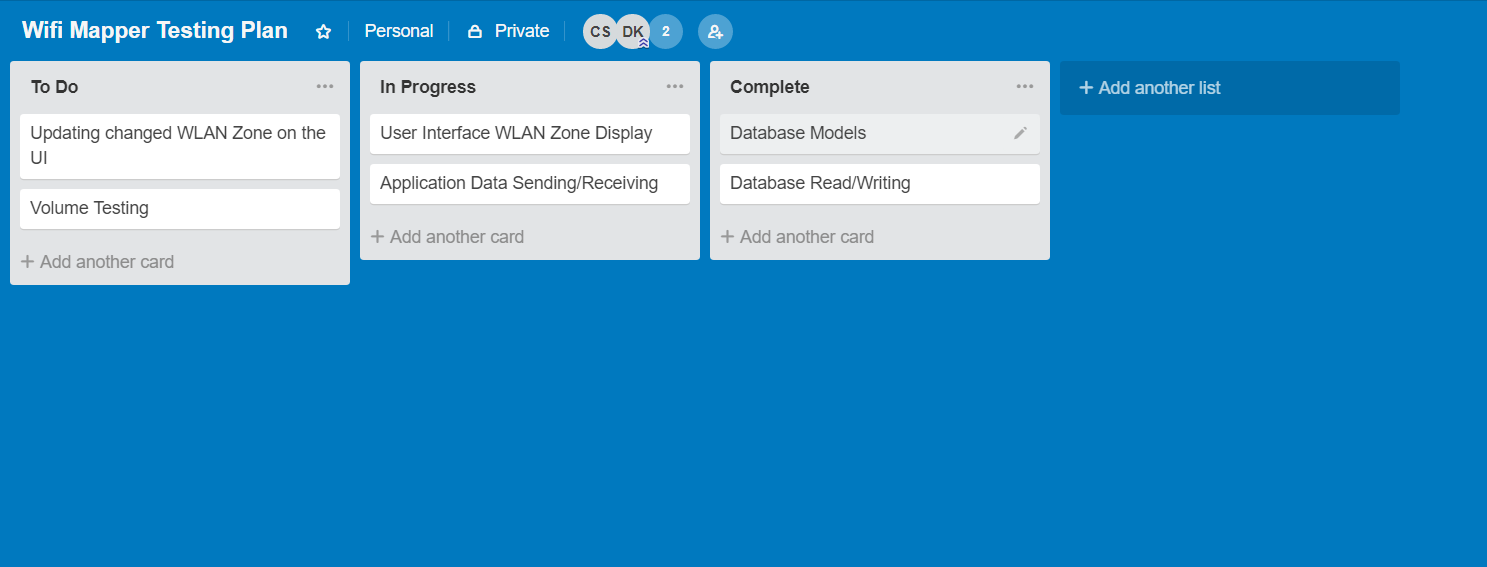
\includegraphics[width=0.7\linewidth]{images/testing_plan}
	\caption{Software management testing plan.}
	\label{fig:testingplan}
\end{figure}
\newpage

\begin{table}[h!]
  \centering
\caption{Summary Testing Plan.}

\begin{tabular}[t]{|p{8cm}|p{7cm}|} \hline

  \textbf{Process} & \textbf{Technique} \\ \hline 1. User Interface Testing: Test view navigation and features & Give user to interact with all the features \\ \hline 2.Database: Test database models and database read and write & Random read and write testing \\
    \hline 3.Volume testing: test application behaviour for large data sets & Random testing of the application with large datapoints \\
    \hline 4. Security and Access Control Testing: test how the application handles privacy & Recovery, security, stress and
    performance tests \\ \hline 5. Failover and Recovery Testing: testing how the application recovers from failure & Recovery, security, stress and
    performance tests  \\ \hline

\end{tabular}

\label{tab:test-plan}
\end{table}

%David
\section{Conclusion}
The goal of the project  was to develop a WiFi Mapper, an app that allows users to view the quality of Eduroam wifi in different WLAN zones at upper campus.

\paragraph{}Our team set out to create a WiFi mapper that would meet the specified user requirements. The features implemented on the app are such that the user can easily determine WLAN zones with the strongest wifi strength.

\paragraph{}This was achieved through the use of different colors on each WLAN zone to depict the strength of the wifi. WLAN zones with different wifi strengths have different colors.The data used to determine the color of the WLAN zone was collected from WiFi routers using the app running in the background.

\paragraph{}Another requirement was that the WiFi mapper should be able to display data on a mobile client and on a web client. Our Wifi mapper managed to do this by having an app running on android devices and on the web. However only the native app is used to collect data from routers.

\paragraph{}The web app only takes data from the database and displays it to the user in the same way the native app does. This allows consistency across the two apps so that the user can have the same experience on both apps. To further meet the requirements that involve user experience, WiFi mapper allows users to zoom and pan on the map as they deem necessary. 

\paragraph{}For advanced like ICTS members of stuff the app allows them to generate a report that shows the perfomance Eduroam accross campus. The report gives numbers of datapoints and number of datapoints collected to the user. It also displays interactive graphs that the user can interact with as the data is collected by the users. The developed app therefore meets most of the requirements that were initially put accross by the client for the users.


%Clayton
x\subsection{User Manual}
\label{ss:user-manual}

Your system must have a user manual. Append this to your report (make
it Appendix A) or bind it separately if it is big. If your system is
interactive and has a good user interface with context dependent help
then this can be just a cheat sheet. Discuss the level at which your
user manual is to be pitched with your client. If your system is to be
extended then you might want to include a technical API manual.


%Meluleki
\section{Conclusion}
\label{sec:conclusion}

This document has covered the major sections needed for your
report. You will probably have each of the subsections 2.1--2.7 as
major section in the report each with its own subsections. 

A marking guide for the report will be provided later.

%David
\section{Code Legibility and Output}

This is not strictly part of the report but is a requirement for the
final hand-in.

\begin{itemize}
\item Each method should start wide a brief description of its
  function.

\item Use indentation to display the structure within a method.

\item Comments should be used extensively. They are best used to
  describe logical blocks of code rather than individual
  statements. Line-by-line comments have the drawbacks of not
  providing any overview and of decreasing readability.

\item Meaningful identifiers should be chosen.

\item Output should be pleasingly formatted and easy to read.
\end{itemize}

You do, of course, have the option to call in any of your
favourite packages for setting maths, graphics, computer listings,
etc.

\begin{thebibliography}{9}

\bibitem[Kopka and Daly(2004)]{KopkaDaly}
Kopka, H. and Daly, P.W.  (2004) \textit{A Guide to \LaTeXe:
Document Preparation for Beginners and Advanced Users} (4th~edn).
Addison-Wesley.

\bibitem[Lamport(1994)]{Lamport}
Lamport L. (1994) \textit{\LaTeX: A Document Preparation System}
(2nd~edn). Addison-Wesley.

\bibitem[Mittelbach and Goossens(2004)]{Companion}
Mittelbach, F. and Goossens, M., (2004) \textit{The \LaTeX\
Companion} (2nd~edn). Addison-Wesley.

\end{thebibliography}
\end{document}
